\documentclass{standalone}

\usepackage{tikz}
\usetikzlibrary{calc}
\usetikzlibrary{arrows.meta}

\begin{document}

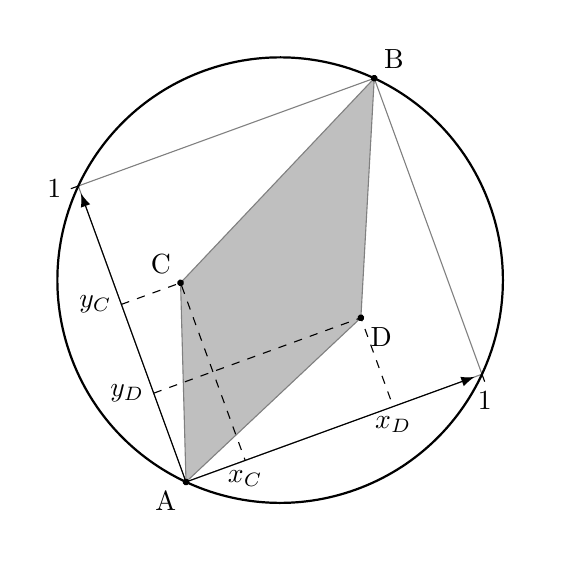
\begin{tikzpicture}[scale=1,rotate=20]

\coordinate[label={below left:A}] (A) at (0,0);
\coordinate[label={above right:B}] (B) at (4,4);
\coordinate[label={above left:C}] (C) at (0.8,2.4);
\coordinate[label={below right:D}] (D) at (2.8,1.2);

\draw[gray, fill=lightgray] (A)--(D)--(B)--(C)--cycle;

\draw[gray] (0,0)--(4,0)--(4,4)--(0,4)--cycle;
\draw[-Latex] (0,0)--(3.9,0);
\draw[-Latex] (0,0)--(0,3.9);

\draw[dashed] (0,2.4) node[left] {$y_C$} -- (0.8,2.4) -- (0.8,0) node[below] {$x_C$};
\draw[dashed] (0,1.2) node[left] {$y_D$} -- (2.8,1.2) -- (2.8,0) node[below] {$x_D$};

\draw (4,0)--++(0,-0.1) node[below] {1};
\draw (0,4)--++(-0.1,0) node[left] {1};

\draw[thick] (2,2) circle (2.8284);
\foreach \pt in {A,B,C,D}{
	\draw[fill=black] (\pt) circle (1pt);
}

\end{tikzpicture}

\end{document}